\newpage
\section{Suggested solutions: $Z$-transform}

\begin{enumerate}
\item Given a discrete time signal $x[n]$, then the $z$-transform is defined as
$$X(z)=\sum_{k=-\infty}^{\infty}x[k]z^{-k}.$$

\begin{enumerate}[a)]

\item Using the definition, we have:
$$X(z)=\mathcal{Z}\{\delta[n]\}=\sum_{k=-\infty}^{\infty}\delta[k]z^{-k}=\delta[0]z^{-0}=1,$$
since the impulse function is only non-zero for $n=0$, for which the value is $1$. 

\item The $z$-transform is linear and for a time-shift, we then have:
\begin{align*}
    X(z)&=\mathcal{Z}\{2\delta[n+4]\}=2\mathcal{Z}\{\delta[n+4]\}, \\
    &=2\sum_{k=-\infty}^{\infty}\delta[k+4]z^{-k}, \\
    &=2z^{4}\mathcal{Z}\{\delta[n]\}, \\
    &=2z^{4},
\end{align*}
since by the previous exercise $\mathcal{Z}\{\delta[n]\}=1$ and by the time-shift theorem. 

\item The $z$-transform of $h[n]=-41\delta[n-42]$ is done in the same way as the previous problem. Skipping the details, we obtain:
$$X(z)=\mathcal{Z}\{-41\delta[n-42]\}=-41z^{-42},$$
again by linearity and the time-shift theorem.

\item For $h[n]=\delta[n+1]-2\delta[n-1]+4\delta[n-4]$ we obtain again by linearity and the time-shift property:
$$X(z)=\mathcal{Z}\{h[n]\}=z^{-1}-2z+4z^{-4}.$$
\end{enumerate}

\item Let the system function for an LTI system be $\mathcal{H}(z)=z^{1}+1+3z^{-1}-0.5z^{-2}+4z^{-10}$.

\begin{enumerate}[a)]

\item If the system function is defined as above, then the impulse response is found by taking the inverse $z$-transform of $\mathcal{H}(z)$. We get:
$$h[n]=\delta[n+1]+\delta[n]+3\delta[n-1]-0.5\delta[n-2]+4\delta[n-10],$$
from this we conclude that the difference equation for the system is:
$$y[n]=x[n+1]+x[n]+3x[n-1]-0.5x[n-2]+4x[n-10],$$
since every LTI system can be expressed as a convolution of the form:
$$y[n]=h[n]*x[n]=\sum_{k=-\infty}^{\infty}h[k]x[n-k],$$
with $h[n]=\mathcal{T}\{\delta[n]\}$. 

\item In Listing \ref{code17_2} is a simple program to plot the impulse response for this system. 
\begin{lstlisting}[language=Python, caption=Code to plot the impulse response function,label=code17_2]
import numpy as n
import matplotlib.pyplot as plt

# sample value we want to plot on
nn = n.array([-2,-1,0,1,2,3,4,5,6,7,8,9,10])

# values for the impulse response function
h = n.array([0,1,1,3,-0.5,0,0,0,0,0,0,0,4])

# plot as a stem plot to emphasize the 
# discrete nature of the function
plt.stem(nn,h)
plt.xlabel("samples [n]")
plt.ylabel("$h[n]$")
plt.title("Impulse response")
plt.show()
\end{lstlisting}
The impulse response plot is shown in Figure \ref{fig17_2}.
\begin{marginfigure}
    \centering
    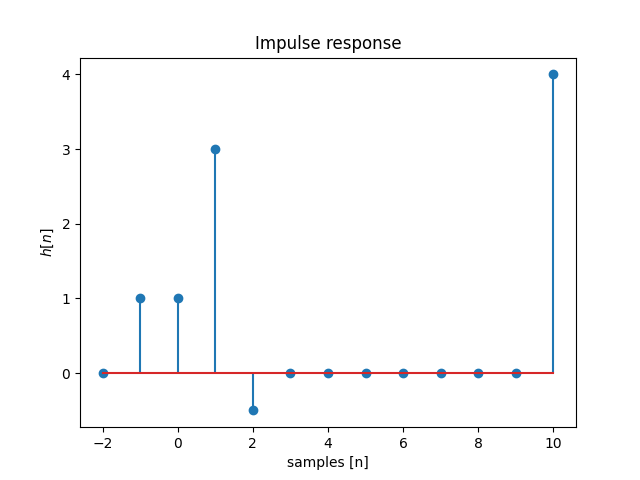
\includegraphics[width=7.5cm,height=7.0cm]{ch18/figures/17_2.png}
    \caption{Output of Listing \ref{code17_2}}
    \label{fig17_2}
\end{marginfigure}

\item If we define a new signal $y_{2}[n]=y[n-2]$, then by the time-shift theorem we have that the new system function will be:
$$Y_{2}(z)=z^{-n_{0}}\mathcal{H}(z)=z^{-2}\mathcal{H}(z)=z^{-1}+z^{-2}+3z^{-3}-0.2z^{-4}+4z^{-12},$$
this new system function will describe a system that is delayed by 2 samples. 
\end{enumerate}

\item Let the system function of a discrete-time LTI system is defined as
$$\mathcal{H}(z)=(z-e^{i\pi/4})(z-e^{-i\pi})z^{-2}.$$

\begin{enumerate}[a)]
\item To determine the effect of this system, factor it:
$$\mathcal{H}(z)=z(1-e^{i\pi}z^{-1})z(1-e^{-i\pi}z^{-1})z^{-2}=(1-e^{i\pi/4}z^{-1})(1-e^{-i\pi}z^{-1}).$$
Then we can view the system function as a cascade of two elementary systems of the form:
\begin{align*}
    \mathcal{H}_{1}(z)&=1-e^{i\pi/4}z^{-1},\\
    \mathcal{H}_{2}(z)&=1-e^{-i\pi}z^{-1}.
\end{align*}
This filter blocks sinusoidal signals of the form $\alpha_{1}=e^{i\pi/4}$ and $\alpha_{2}=e^{-i\pi}$, which correspond to normalized angular frequencies of $\hat{\omega}=\pi/4,-\pi$. 

\item The poles and zeros of the system function is shown in Figure \ref{z:ex3}. 

\begin{marginfigure}[-5cm]
\begin{center}
\begin{tikzpicture}
	\begin{axis}[axis equal, ymin=-1.5,xmin=-1.5,ymax=1.5,xmax=1.5,  ticks=none,
    xlabel=$\mathrm{Re}(z)$,
    ylabel=$\mathrm{Im}(z)$, axis lines = middle, width=7cm, height=7cm]
	\addplot [gray,domain=0:2*pi,samples=50]({cos(deg(x))},{sin(deg(x))});

\addplot [blue, mark = o,mark size=3pt] coordinates {({cos(45)}, {sin(45)})} {};   
\addplot [blue, mark = o,mark size=3pt] coordinates {({cos(180)}, {sin(180)})} {};  
\addplot [red, mark = x,mark size=3pt] coordinates {({0}, {0})} {}; 
\end{axis}
\end{tikzpicture}
\end{center}
\caption{The zeros of the system function $\mathcal{H}(z)$,
have $\alpha_k=\{e^{i\pi/4},e^{-i\pi}\}$. Zeros are marked with blue
    circles and poles are marked with red crosses.}
\label{z:ex3}
\end{marginfigure}

\item 


\end{enumerate}


\end{enumerate}